\section{The MTMR system}
MTMR implements MapReduce for traditional HPC systems such as 
supercomputers. Its goal is to enable efficient big data processing
at large scale.


\subsection{MTMR runtime design}

The MTMR is developed using C++, MPI, and OpenMP. It uses OpenMP to
enable multithreaded processing in map and reduce functions. It uses 
non-blocking MPI collectives to communicate $\langle key, value \rangle$ pairs 
between map and reduce phases, and to overlap communication
with map computation. 

With the goal of optimizing the shuffle stage performance,
there are two main design choices that we used. First, our library adapted
a multithreaded model for map and reduce functions. Second, 
we used non-blocking MPI collectives to overlap communication
and computation. We briefly introduce them here and discuss them in
details in the following sessions.

Comparing to the MapReduce-MPI which runs one MPI process
on each computing core, our library runs one MPI process on each
computing node, and uses OpenMP to take advantage of intra-node
parallelism. The reasoning behind this decision is to improve
the performance of the all-to-all communication in the shuffle stage.
As shown in Figure~\ref{}, the performance of the MPI\_Alltoallv 
is improved in the case of using one process on each node than 
using one process on each core when communicating the same
amount of data that follows the same node-to-node communication
pattern. To use MPI\_Alltoallv more efficiently, we adopt this one
process per node pattern, and use multiple threads to execute map
and reduce functions.

Moreover, with the support of non-blocking collective in MPI, it
enables library writers to overlap communication and computation 
easily. Our library starts communicating $\langle key, value \rangle$ pairs 
as soon as the first memory buffer which stores the the $\langle key, value \rangle$
pairs is full, this allows our system to overlap communication
and computation efficiently.

Figure~\ref{overview_mtmr} shows the comparison of our 
Multithreaded MapReduce library with the MapReduce-MPI library.
As discussed in Section~\ref{background}, the shuffle stage
can be divided into two steps: communication and reorganization. The 
communication step sends and receives $\langle key, value \rangle$  pairs. 
The reorganization step gathers all the values associated with
the same key (the values may come from different processes) and 
forms the input to reduce. 
n MapReduce-MPI, the
shuffle phase starts after the map phase, and finishes before the
reduce phase. In comparison, our library pushes the communication
step of the shuffle into the map phase, and combines the reorganization
step with the reduce phase.
\begin{figure}[!htb]
\centering
  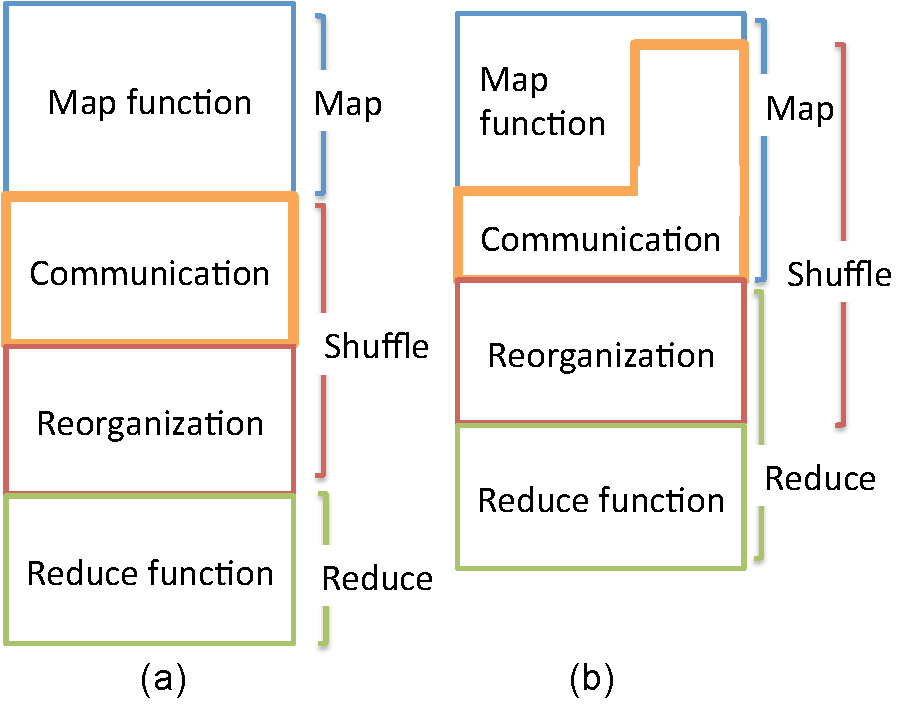
\includegraphics[width=0.9\linewidth,height=2.2in]{figs/overview_mtmr.pdf}
  \caption{MapReduce operations: map, shuffle, and reduce operations in a
  typical MapRedue runtime such as MapReduce-MPI (a); and map, shuffle, and
  reduce operations in our MTMR runtime (b).}
  \label{fig:overview_mtmr}
\end{figure}

\subsection{Design of multithreaded map}

Key points:
\begin{itemize}
\item double buffers for (1) work sharing among threads (2) non-blocking 
communication
\item how to handle thread synchronization when using double buffers,
use atomic fetch and add operation, use local buffer per thread
\item improvements and advantages over MRMPI (or Hadoop)
\end{itemize}

The overall process of map is presented in Figure~\ref{fig:multithreaded_map}.  
The map process reads initial input into a memory buffer and stores them as
data records. We denote the memory buffer which stores the
data records by $BUFF_{input}$. The input can be broken up into records
in multiple ways. Currently, our library supports two types of
data records. In the first type, each data record is a English
word; while in the second type, each data record is one line
of text in the input.
\begin{figure*}[!htb]
\centering
  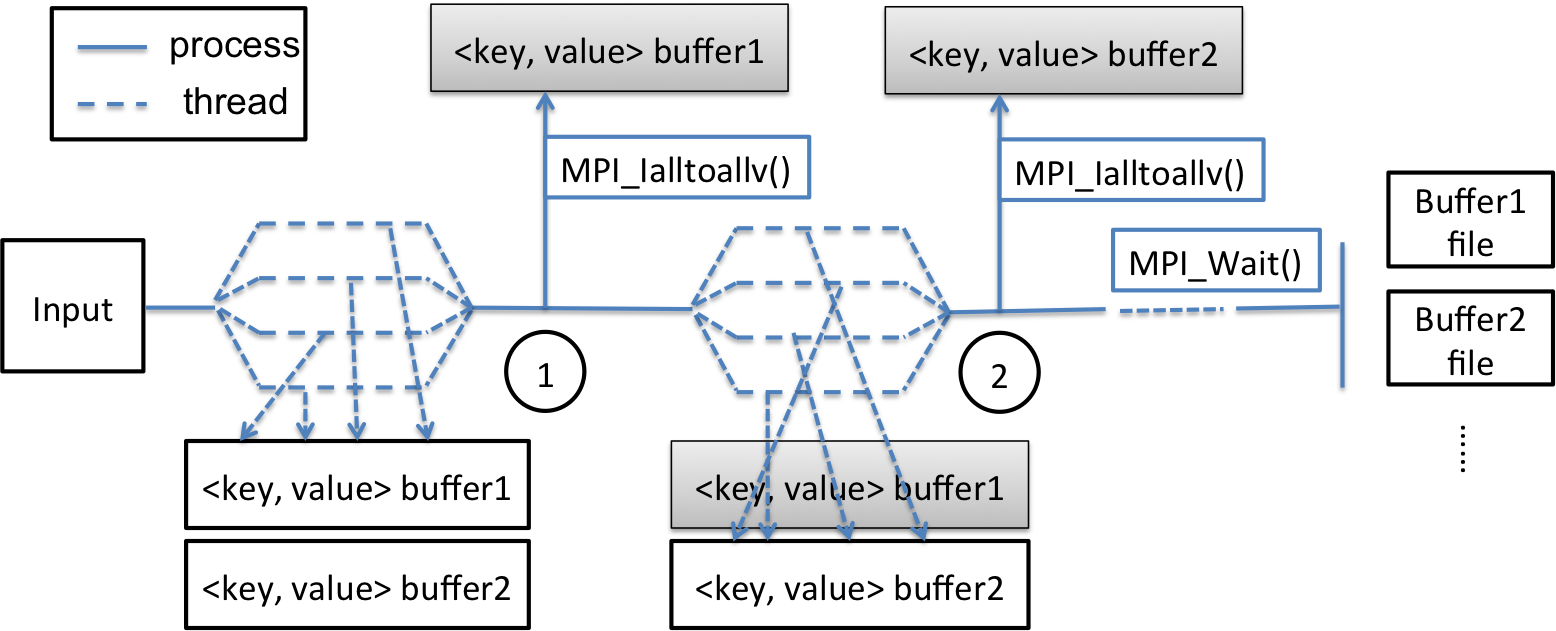
\includegraphics[width=0.8\linewidth,height=2.2in]{figs/multithreaded_map_design.png}
  \caption{Design of multithreaded Map phase.}
  \label{fig:multithreaded_map}
\end{figure*}

When the $BUFF_{input}$ is full, the process starts an 
OpenMP session in which
each thread reads a subset of data records from the $BUFF_{input}$, applies the user
defined map function to each record, generates
the intermediate $\langle key, value \rangle$ paris, and stores the intermediate
$\langle key, value \rangle$ pairs collectively into a second memory.
We denote the second memory buffer by $BUFF_{kv1}$.
$BUFF_{kv1}$ is used for two purposes. First, it stores
the intermediate output for each map process. Second,
it is used as the send buffer in the subsequent MPI\_Ialltoallv()
to communicate the intermediate data.

There are two important aspects that we need to consider.
First, in order to use $BUFF_{kv1}$ as the send buffer in MPI\_Ialltoallv(),
all the intermediate pairs that need to be sent to process $p_{i}$ need
to be stored in a continuous region. To this end, we partition
the $BUFF_{kv1}$ into n regions of the same size, n is the number
of process running. Then we apply a hash function to determine
the destination process of the intermediate pair and store
the pair in corresponding region of $BUFF_{kv1}$. 
We use an additional array to keep track of location in $BUFF_{kv1}$
to store the next pair. Figure~\ref{fig:map_data_structures}(a) shows
the $BUFF_{kv1}$ after partition when there are four processes,
and Figure~\ref{fig:map_data_structures} shows the corresponding OFFSET array
that stores the location to write the next intermediate pair.
\textbf{write something about the hash function, give ref}
\begin{figure}[!htb]
\centering
  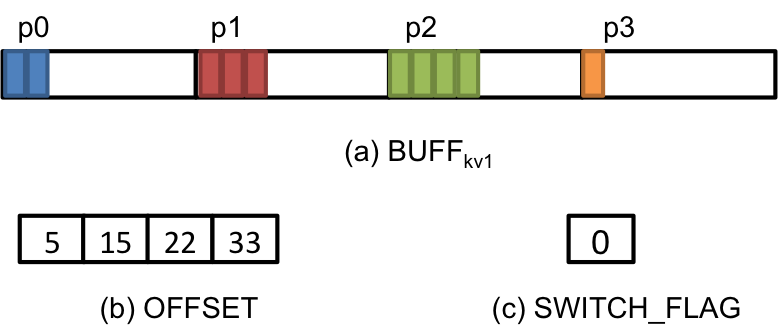
\includegraphics[width=0.9\linewidth,height=1.2in]{figs/map_data_structures.png}
  \caption{MapReduce operations: map, shuffle, and reduce operations in a
  typical MapRedue runtime such as MapReduce-MPI (a); and map, shuffle, and
  reduce operations in our MTMR runtime (b).}
  \label{fig:map_data_structures}
\end{figure}

Second, in order to avoid data race when multiple threads
try to write to the same buffer location,  and to ensure all threads exit
the parallel session in case any section of the $BUFF_{kv1}$ overflows, 
we need to ensure efficient synchronization. To this end, 
we use atomic operation $fetch\_and\_add$ as shown in
Algorithm~\ref{ag:sync_map}, and
a boolean variable named SWITCH\_FLAG as shown in 
Figure~\ref{fig:map_data_structures}(c).
$SWITCH\_FLAG  = false$ means it is OK to write the current
intermediate pair to $BUFF_{kv1}$ without overflowing it. Otherwise,
it means writing the current pair will overflow $BUFF_{kv1}$, and 
all threads should exit the parallel session, and $BUFF_{kv1}$ 
needs to be communicated using MPI\_Ialltoallv().
\begin{algorithm}
\caption{Synchronization in Multithread Map}
\label{ag:sync_map}
\begin{algorithmic}[1]
\While{$left > 0$}
\State \#pragma opm parallel
\State \{
\While{  $left_{me} > 0$ \&\& $!SWITCH\_FLAG$}
\State $\langle key, value \rangle \gets map(record)$
\State $offset \gets fetch\_and\_add(\&offset[i], size)$
\If{$offest + size < limit$}
\State copy $\langle key, value \rangle$ to $BUFF_{kv1}$
\State $myDone\mathrel{++}$
\Else
\State $SWITCH\_FLAG = true$
\EndIf
\EndWhile
\State \}
\State \#pragma omp atomic
\State $left \mathrel{-}= myDone$
\EndWhile
\end{algorithmic}
\end{algorithm}

In Algorithm~\ref{ag:sync_map}, $left$ is the number of data record
that need to be processed in $BUFF_{input}$. When there exists 
some data records need to be processed, we start a parallel session.
Each thread keeps track of the number of data record it needs to
process (local variable $left_{me}$), and reads the value of SWITCH\_FLAT
which is a global variable. If the both conditions are met, i.e., the
thread has some number of data records to process, and the
$BUFF_{kv1}$ is not overflowed, the thread calls the user
defined map function, reserves storage space in the $BUFF_{kv1}$
by calling $fetch\_and\_add$. The it tests to see if by copying 
the intermediate pair will overflow the $BUFF_{kv1}$, if not,
the intermediate pair is copied to $BUFF_{kv1}$, otherwise,
the overflow buffer flag $SWITCH\_FLAG$ is set to true.

We can validate the correctness of this algorithm by considering
the following scenarios. Hypothetically, we have four processes
in the system, and each process runs two threads (i.e. $T0$ and $T1$). The following 
four scenarios cover all possible execution paths that may
cause a data race or a buffer overflow. Due to space limitation,
we list the scenarios here, and leave the details of walking through 
the algorithm to the readers.

\begin{itemize}
\item Two threads try to write to different sections of $BUFF_{kv1}$,
$T0$ overflows the buffer, and $T1$ does not.
\item Two threads try to write to different sections of $BUFF_{kv1}$,
both overflow the buffer.
\item Two threads try to write to same sections of $BUFF_{kv1}$,
$T0$ overflows the buffer, and $T1$ does not.
\item Two threads try to write to same sections of $BUFF_{kv1}$,
both overflow the buffer.
\end{itemize}

We realize that the frequent calls to the atomic
$fetch\_and\_add$ is the bottleneck for performance and apply
further optimization by introducing a thread local memory
buffer to hold intermediate $\langle key, value \rangle$ pairs.
The thread local memory buffer has a similar structure as
shown in Figure~\ref{fig:mao_data_structures}(a), but much
smaller in size (\textbf{give numbers}). Each thread writes
to its local buffer first without the need to use atomic
operations, only when its local buffer overflows, the thread
calls $fetch\_and\_add$ to reserve space in the process 
owned global buffer $BUFF_{kv1}$. The process requires 
only minor changes to Algorithm~\ref{ag:syn_map}. 

Continue with the map processing, after having enough 
intermediate pairs that eventually make $BUFF_{kv1}$ overflow,
the threads exit the parallel session collectively. At this point,
the process communicates the $BUFF_{kv1}$ using 
non-blocking $MPI\_Ialltoallv()$, and immediately continues to process 
data records in $BUFF_{input}$ that are left.
This time, the threads stores intermediate pairs in a third 
memory buffer named $BUFF_{kv2}$ as shown in Figure~\ref{fig:multithreaded_map}.
This operation of multithreaded mapping and storing intermediate
data to a memory buffer (either $BUFF_{kv1}$ or $BUFF_{kv2}$), and
communicating of the full memory buffer among processes
repeat until all the input files are exhausted. The we
wait for all the previous $MPI\_Ialltoallv()$ to return using $MPI_Wait()$
before moving on to the reduce phase. 
 
The use of double buffering serves both purposes of working sharing
among threads, and the send buffer for communication. It 
brings several merits including


The key idea of the design is to use one process on each node to ensure
node to node communication (instead of multiple communication channels
among two nodes), and to use multiple threads to apply the map function
to generate the intermediate key value pairs. To enable the design, we 
use two buffers (double buffer, overflow buffer?) to hold intermediate 
key value pairs for the direct communication among processes (nodes), without
spilling on disk file (which is the case of MR-MPI).

In the map function, the process first reads the input
file into the memory buffer \textit{in\_buffer}, (called \textit{in\_buffer}, size is configureable 
by the user). At the same time, each process
maintains two memory buffers (named \textit{kv\_buffer1} and \textit{kv\_buffer2}) 
to store the intermediate output of map function. After the \textit{in\_buffer} is
populated with data records, the program spawns an OpenMP parallel
session, in which each thread reads a distinct part of the data records
in \textit{in\_buffer}, applies the user defined map function, and writes the
intermediate output to the \textit{kv\_buffer} collectively. When the 
\textit{kv\_buffer} is full, it is used as the MPI send buffer in the non-blocking
MPI\_Ialltoallv communication to send key value pairs. 

---

The benefits are:


\subsection{Multithreaded reduce}

Key point:
\begin{itemize}
\item almost entirely multithreaded
\item use dictionary and hash table to reorganize 
\end{itemize}

The use of dictionary and hash table are suggested by yanfei, need to point out.
The reduce phase is almost entirely multithreaded. The reduce phase starts
by reorganizing the $\langle key, value \rangle$ pairs received in one buffer to group
all the values associated with the same key. Then the reduce phase
reorganizes the pairs across all the buffers received from the map phase.




